\documentclass{bmvc2k}

%% Enter your paper number here for the review copy
% \bmvcreviewcopy{??}

%\usepackage[brazilian]{babel}
\usepackage[utf8]{inputenc}

\title{Projeto Demonstrativo 1}

% Enter the paper's authors in order
% \addauthor{Name}{email/homepage}{INSTITUTION_CODE}
\addauthor{Pedro Henrique Luz de Araujo}{pedrohluzaraujo@gmail.com}{1}

% Enter the institutions
% \addinstitution{Name\\Address}
\addinstitution{
  Departamento de Ci\^encia da Comptuta\c{c}\~ao\\
  Universidade de Bras\'{\i}lia\\
  Campus Darcy Ribeiro, Asa Norte\\
  Bras\'{\i}lia-DF, CEP 70910-900, Brazil,  
}

\runninghead{Luz de Araujo, P.H.}{Projeto Demonstrativo 1 -- \today}

% Any macro definitions you would like to include
% These are not defined in the style file, because they don't begin
% with \bmva, so they might conflict with the user's own macros.
% The \bmvaOneDot macro adds a full stop unless there is one in the
% text already.
\def\eg{\emph{e.g}\bmvaOneDot}
\def\Eg{\emph{E.g}\bmvaOneDot}
\def\etal{\emph{et al}\bmvaOneDot}

%-------------------------------------------------------------------------
% Document starts here
\begin{document}
\begin{NoHyper}
\maketitle
\end{NoHyper}

\begin{abstract}
O presente Projeto Demonstrativo consiste em um programa capaz de: informar posição e valor de um pixel escolhido tanto em imagens coloridas quanto em escala de cinza; e colorir todos os pixeis de uma imagem ou vídeo, capturado em tempo real ou não, cujo valor seja próximo ao de um pixel selecionado. O projeto divide-se em quatro requisitos: o primeiro trata da obtenção das coordenadas e valores de pixeis; o segundo, da colorização de pixeis semelhantes de uma imagem; o terceiro é análogo ao segundo, mas em vídeo; por fim, o quarto é equivalente ao terceiro aplicado a uma captura de vídeo em tempo real.
\end{abstract}

%-------------------------------------------------------------------------
\section{Introdução}
\label{sec:intro}
O Projeto Demonstrativo 1 tem como objetivo estabelecer o primeiro contato com técnicas de processamento de imagem e vídeo que serão usadas em aplicações de Visão Computacional. Tais aplicações buscam reconstruir propriedades visuais do mundo (forma, iluminação, distribuição de cores) a partir de uma ou mais imagens~\cite{Szeliski:2010:CVA:1941882}. Como ponto de partida, foram explorados o carregamento de imagens e vídeos e a representação computacional das cores.

As imagens podem ser representadas digitalmente como matrizes tridimensionais, em que duas das dimensões representam a posição dos pixeis, enquanto a outra representa a cor de cada pixel. Um vídeo por sua vez, pode ser considerado uma sequência de imagens, onde cada uma representa um \textit{frame} do vídeo.

Já as cores são comumente representadas por três \textit{bytes}, no caso de imagens coloridas, ou apenas um \textit{byte} no caso de imagens em preto e branco. No primeiro caso, cada um dos \textit{bytes} corresponde a intensidade de uma cor primária. No espaço de cores RGB, por exemplo, cada \textit{byte} representa a intensidade de vermelho, verde ou azul. No segundo caso, 0 representa preto, 255, branco, e os valores intermediários são tons de cinza. Dessa forma, é possível estabelecer uma medida de semelhança entre cores, por exemplo, por meio da distância euclidiana entre elas no espaço de cores

O presente trabalho está organizado da seguinte maneira: a Seção \ref{sec:met} apresenta a metodologia utilizada para a construção do programa; a Seção \ref{sec:res} apresenta os resultados obtidos; e a Seção \ref{sec:disc} conclui o trabalho.

\section{Metodologia}
\label{sec:met}
\subsection{Ferramentas}
\label{subsec:fer}
Usamos a biblioteca OpenCV~\cite{opencv_library} para o carregamento e exibição de imagens e vídeos. Para realizar operações sobre as matrizes de imagens, utilizamos a biblioteca NumPy. Usamos ainda, como linguagem, Python 3.5.2, e o gerenciador de bibliotecas Anaconda 3.

\subsection{Implementação e Uso}
\label{subsec:imp}
Para o carregamento e exibição de imagens e vídeos, bastou a utilização de funções da biblioteca OpenCV. O usuário tem como opção usar imagens padrão guardadas na pasta \textit{data} ou utilizar imagens próprias, conforme instruções presentes no arquivo \textit{read-me.txt}.

O requisito 1 trata do carregamento e apresentação de uma imagem na tela. O usuário pode clicar na imagem e obter no terminal as coordenadas e o valor do pixel clicado. Em caso de imagens coloridas, tal valor é uma tripla de inteiros que representam a intensidade de vermelho, verde e azul; em imagens em tons de cinza, trata-se apenas de um inteiro. Ressaltamos que a biblioteca OpenCV representa as cores em BGR, o inverso de RGB, de modo que mostrou-se necessário inverter a tripla ao apresentá-la ao usuário.

O requisito 2 permite que o usuário clique em um pixel de modo que todos os outros pixeis com cor ``semelhante'' à dele são coloridos de vermelho. Foi estabelecida como medida de semelhança a distância euclidiana no espaço de cores. Definiu-se que pixeis semelhantes apresentam distância menor que 13. A distância euclidiana foi calculada utilizando a biblioteca de álgebra linear do NumPy, em razão de sua implementação otimizada.

O requisito 3 aplica a técnica do requisito 2 a vídeos. A diferença principal é a necessidade de colorir cada um dos \textit{frames}. Por fim, o requisito 4 é análogo ao requisito 3, mas aplicado a vídeos obtidos em tempo real.

\section{Resultados}
\label{sec:res}
\subsection{Requisito 1}
A figura \ref{fig:requisto 1} apresenta a imagem carregada e analisada e o retorno ao usuário após clicar, respectivamente, nos cantos superior esquerdo, superior direito, inferior esquerdo e inferior direito da imagem, e nas partes com cor vermelha, verde e azul. Tais experimentos indicam o funcionamento correto do procedimento

\begin{figure}[htb]
  \centering
  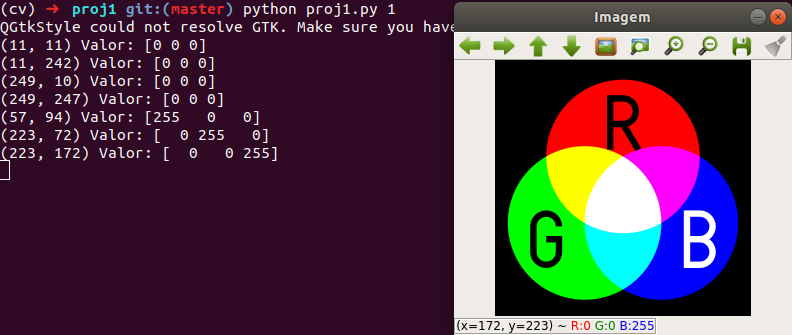
\includegraphics[width=0.9\linewidth]{Figs/requisito1.png}
  \caption{Imagem~\cite{wiki:requisito1} analisada e exibição de coordenadas e valores dos pixeis clicados.}
  \label{fig:requisto 1}
\end{figure}

\subsection{Requisito 2}
As figuras \ref{fig:original} e \ref{fig:red_original} comparam a imagem original antes e depois de clicar nas partes pretas e azul. Ao clicar no preto, tudo que é preto tornou-se vermelho; ao clicar no azul, o azul tornou-se vermelho.

\begin{figure}[htb]
	\label{}
    \centering
    \begin{minipage}{0.45\textwidth}
        \centering
        
\includegraphics[width=0.9\textwidth]{Figs/default_image.png}
        \caption{Figura original.}
        \label{fig:original}
    \end{minipage}\hfill
    \begin{minipage}{0.45\textwidth}
        \centering
        
\includegraphics[width=0.9\textwidth]{Figs/vermelho.png}
        \caption{Figura após edições.}
        \label{fig:red_original}
    \end{minipage}
\end{figure}

As figuras \ref{fig:lena} e \ref{fig:red_lena}, e \ref{fig:pavão} e \ref{fig:red_pavão} exibem o funcionamento do requisito 2 em uma imagem em preto e branco e em uma imagem com intensa nuance de cores, respectivamente.

\begin{figure}[htb]
    \centering
    \begin{minipage}{0.45\textwidth}
        \centering
        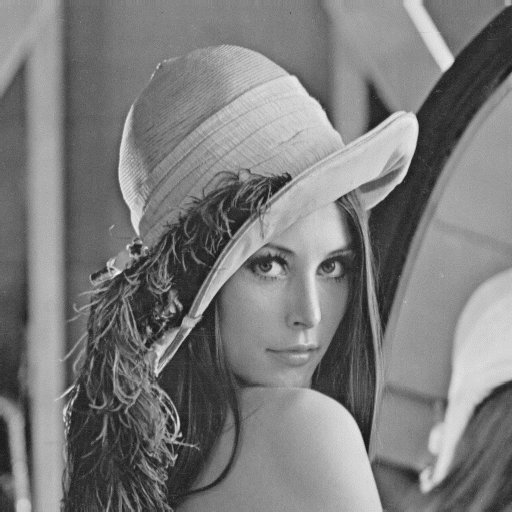
\includegraphics[width=0.9\textwidth]{Figs/lena.png}
        \caption{Figura original.}
        \label{fig:lena}
    \end{minipage}\hfill
    \begin{minipage}{0.45\textwidth}
        \centering
        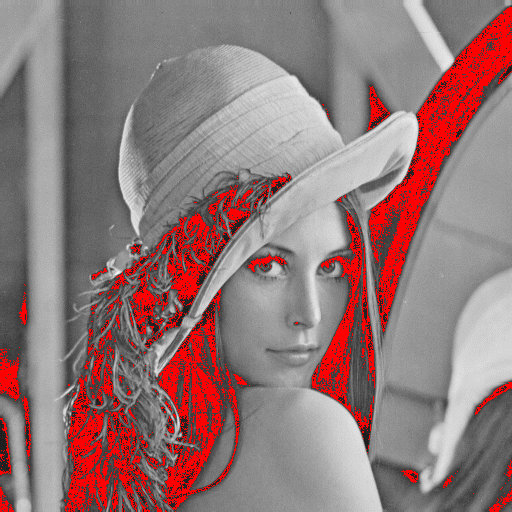
\includegraphics[width=0.9\textwidth]{Figs/red_lena.png}
        \caption{Após clicar nas penas.}
        \label{fig:red_lena}
    \end{minipage}
\end{figure}

\begin{figure}[htb]
    \centering
    \begin{minipage}{0.45\textwidth}
        \centering
        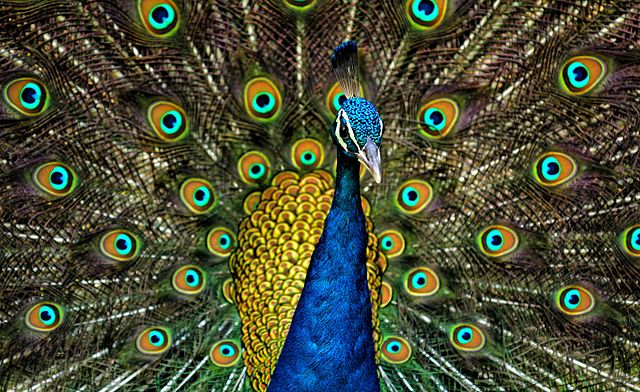
\includegraphics[width=0.9\textwidth]{Figs/peacock.jpg}
        \caption{Figura original~\cite{wiki:pavao}.}
        \label{fig:pavão}
    \end{minipage}\hfill
    \begin{minipage}{0.45\textwidth}
        \centering
        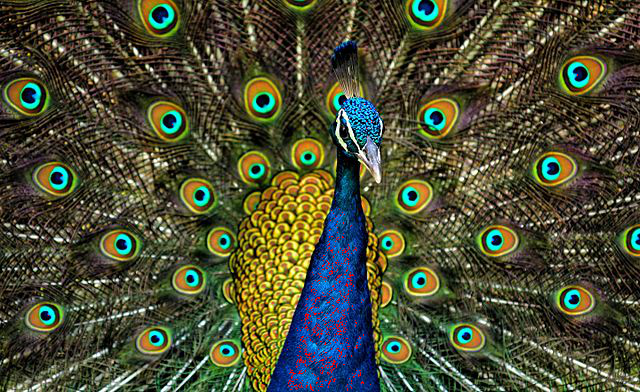
\includegraphics[width=0.9\textwidth]{Figs/red_peacock.png}
        \caption{Após clicar no pescoço.}
        \label{fig:red_pavão}
    \end{minipage}
\end{figure}

\subsection{Requisito 3}
A figura \ref{fig:red_drop} exibe um \textit{frame} do vídeo padrão do requisito 3~\footnote{Retirado do site \href{http://www.engr.colostate.edu/me/facil/dynamics/avis.htm}{http://www.engr.colostate.edu/me/facil/dynamics/avis.htm}, acesso em 26 de agosto de 2018}, que consiste em uma gota caindo em água, após um clique. Na execução do requisito, os \textit{frames} são colorizados e atualizados em tempo real à medida em que o vídeo progride.

\begin{figure}[!htb]
  \centering
  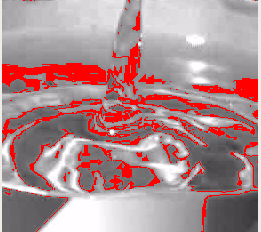
\includegraphics[width=0.5\linewidth]{Figs/red_drop.png}
  \caption{\textit{Frame} após colorização.}
  \label{fig:red_drop}
\end{figure}

\subsection{Requisito 4}
A figura \ref{fig:red_me} consise em um \textit{frame} de uma captura por \textit{webcam} após o clique em um pixel do vídeo. Assim como no caso do requisito 3, os \textit{frames} são colorizados em tempo real durante a captura do vídeo. 

\begin{figure}[!htb]
  \centering
  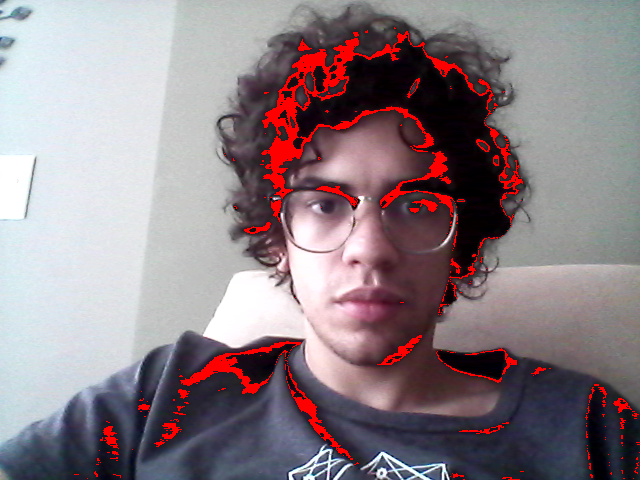
\includegraphics[width=0.5\linewidth]{Figs/red_me.png}
  \caption{\textit{Frame} após colorização.}
  \label{fig:red_me}
\end{figure}

\section{Discussão e Conclusões}
\label{sec:disc}
O presente trabalho demonstrou o processo de carregamento e exibição de imagens e vídeos usando a biblioteca OpenCV, além da manipulação individual dos pixeis de uma imagem ou \textit{frame} por meio da biblioteca NumPy.

Primeiramente, ficou clara durante a implementação da aplicação a necessidade de vetorização do procedimento de colorização das imagens. Embora um \textit{loop} por todos os pixeis seja viável na colorização das imagens, o mesmo não se aplica ao caso dos vídeos, que apresentam vários \textit{frames} a serem processados por segundo. Daí a importância do uso das operações sobre matrizes implementadas pelo NumPy, que são otimizadas.

Além disso, ao se comparar a colorização da imagem \ref{fig:pavão} com as demais, nota-se que poucos pixeis foram colorizados. Tal fato se deve à grande variedade de cores da imagem. Para conseguir um bom resultado na colorização dela seria necessário aumentar a distância máxima para se considerar duas cores semelhantes.

O código-fonte do projeto está disponível em \href{https://github.com/peluz/cv-foundations-1}{https://github.com/peluz/cv-foundations-1}.

\bibliography{refs}
\end{document}
